%!TEX root = Lefley - Mesh to voxel transformations for optimised physics-based interactions.tex
\chapter{Evaluation}

This chapter will investigate the success of Dynamic Volumetric Fragmentation as a solution for computing the destructive results of physics-based collisions. Visual evaluation of the results produced will be carried out as well as empirical comparison with another destruction library for Unity3D.

Further work which could be done to improve the solution as it is in its current state will also be discussed.

\section{Comparison}

The `Meshinator' library available for Unity3D will be used for comparative evaluation\cite{Meshinator}. This library also fractures objects dynamically based on impact force and user defined object strength, however the method differs from ours.

Meshinator performs fragmentation by intersecting a plane, positioned depending on the impact force and object strength, with the object and shearing along it. Triangles crossing the plane are clipped to it and the two resulting meshes are closed with a flat surface. This can be seen in Figure~\ref{fig:4.1}.

\begin{figure}
\centerline{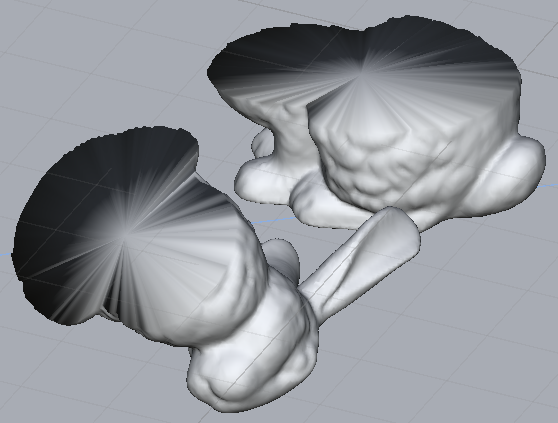
\includegraphics[scale=0.75]{fracture_bunny.png}}
\caption{The Stanford Bunny fractured into two fragments by the `Meshinator' library.}
\label{fig:4.1}
\end{figure}

\subsection{Advantages}

\subsubsection{Latency}

As will be seen in Section~\ref{sect:emp}, the Meshinator library has a lower latency between the start and end of the fracturing pipeline. The reasons for this will be explored in further detail.

\subsubsection{Conservation of volume}

Due to the mesh being partitioned exactly by a plane, none of the original mesh's volume is lost on fragmenting. This is not the case with Dynamic Volumetric Fragmentation for two reasons:

\begin{itemize}
\item{Triangles from the original mesh are lost rather than clipped during mesh partitioning. See Section~\ref{sect:part}.}
\item{When applying marching tetrahedra to two adjacent volumes, there will be a gap between the two resulting meshes.}
\end{itemize}

With our method, volume loss is minimised with increased triangle density in the original mesh as well as voxel resolution, at a computational cost. This is shown in Figures \ref{fig:4.2} and \ref{fig:4.3}.

\begin{figure}
\centerline{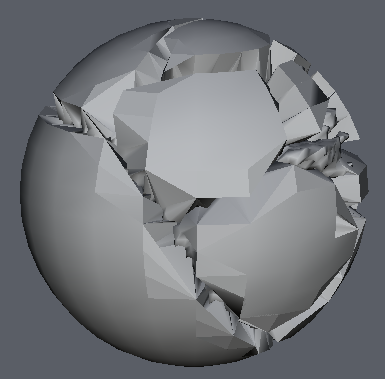
\includegraphics[scale=0.8]{voxel_sphere.png}}
\caption{The sphere has a low triangle count and so when the original mesh is partitioned and triangles are lost, a larger volume is lost in the end result.}
\label{fig:4.2}
\end{figure}
\begin{figure}
\centerline{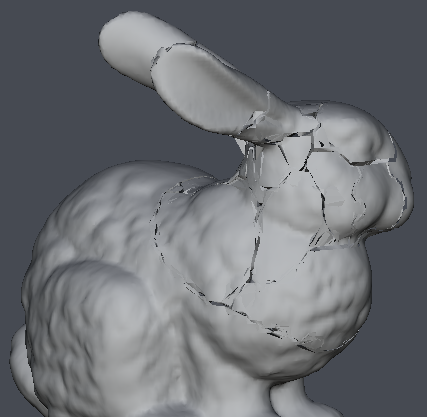
\includegraphics[scale=0.75]{voxel_bunny.png}}
\caption{The Stanford Bunny has a higher triangle count and so less volume is lost in the end result.}
\label{fig:4.3}
\end{figure}

\subsection{Disadvantages}

The following are some limitations of the Meshinator library compared to Dynamic Volumetric Fragmentation.

\subsubsection{Concavities}

As discussed in Section~\ref{sect:prob}, Meshinator cannot correctly fracture objects with concave sections. This is because of how the shearing is implemented. All of the vertices created by clipping triangles to the plane are added to new triangles in pairs with the third vertex being a point at the centre of the bounding box around these vertices. The result of this is shown in Figures \ref{fig:4.4} and \ref{fig:4.5}. DVF does not have this limitation for the reasons discussed in Section~\ref{sect:sol}.

\begin{figure}
\centerline{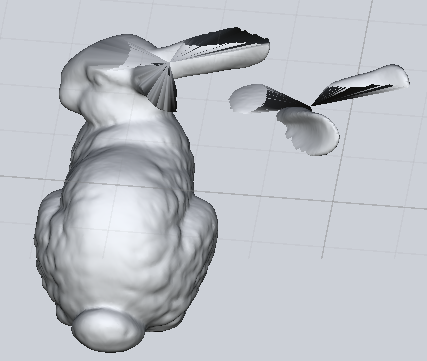
\includegraphics[scale=1]{fracture_non_concave.png}}
\caption{The incorrect fragments generated when Meshinator shears across a concavity.}
\label{fig:4.4}
\end{figure}
\begin{figure}
\centerline{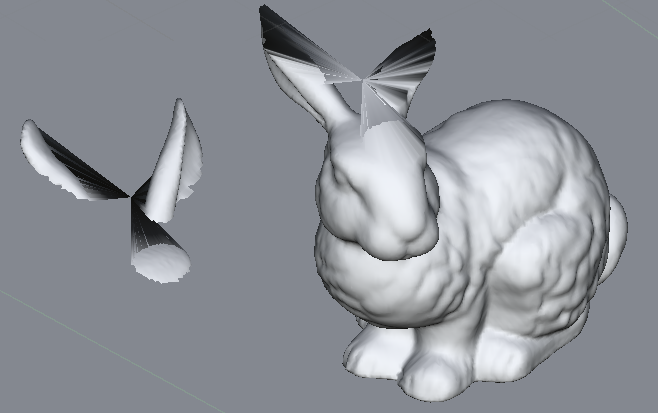
\includegraphics[scale=0.75]{fracture_non_concave2.png}}
\caption{The incorrect fragments generated when Meshinator shears across a concavity. Seen from another angle.}
\label{fig:4.5}
\end{figure}

\clearpage
\subsubsection{Accuracy}

\label{sect:acc}

The visual accuracy of the Meshinator library is limited as it is only able to create flat planar shears when fragmenting. This is only physically accurate for some materials such as crystal. DVF allows for the partitioning pipeline stage to be easily swapped depending on the desired material properties, with the presence of the volume data giving a high number of possibilities.

Also, the Meshinator library always produces the same shear under the same impact, which is not realistic. Due to the distribution of the Voronoi generating points, DVF gives varied results under the same forces. This gives the realistic impression that no two objects are truly exactly the same. A comparison can be seen in Figures \ref{fig:4.6} and \ref{fig:4.7}.

\begin{figure}[b!]
\centerline{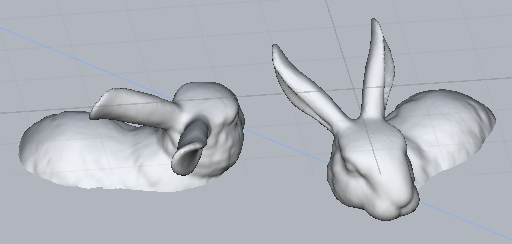
\includegraphics[scale=0.8]{fracture_same_shape.png}}
\vspace{0.1in}
\centerline{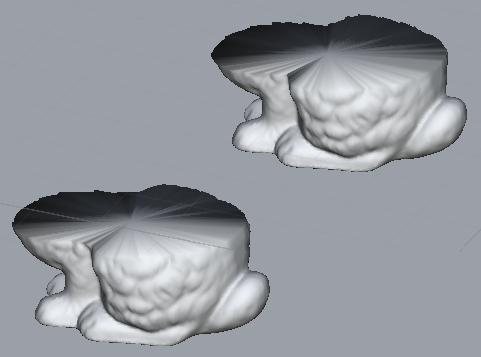
\includegraphics[scale=0.85]{fracture_same_shape2.png}}
\caption{When two identical objects are fragmented under the same forces using Meshinator the results are also identical.}
\label{fig:4.6}
\end{figure}
\begin{figure}
\centerline{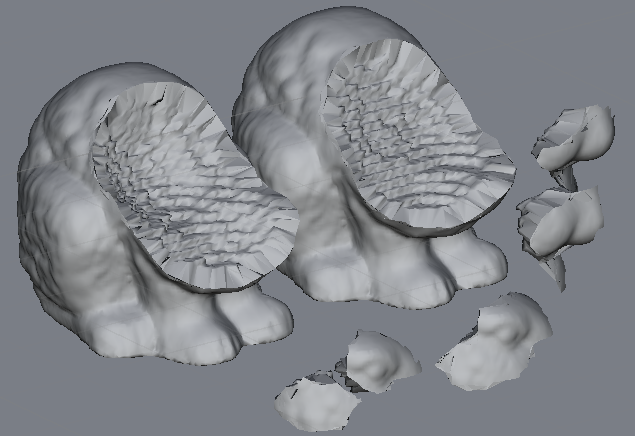
\includegraphics[scale=0.7]{voxel_different.png}}
\caption{When two identical objects are fragmented under the same forces using this solution the results vary slightly as they would in the real world.}
\label{fig:4.7}
\end{figure}

\section{Empirical Evaluation}

\label{sect:emp}

The main focus of this project was to investigate a solution which enables physically accurate object fragmentation. However, testing the physical accuracy implemented by the current partitioning pipeline stage empirically is beyond the scope of the project. Limitations exist in the Voronoi based partitioning as well as in the meshing stage with regards to physical accuracy. These problems, as well as whether the project is a viable starting point for more accurate fragmentation algorithms to be used in will be discussed in Section~\ref{sect:accurate}.

Instead, comparative empirical evaluation will be done between the Meshinator library and this implementation regarding use as a real-time solution for physical destruction.

\subsection{Metrics}

The following metrics are used for evaluation.

\subsubsection{Latency}

The delta time from the start of the fragmentation process to the end. In the case of Dynamic Volumetric Fragmentation this has been split for each pipeline stage.

This is the most important metric as the destructible object cannot visually fragment until the fragmentation stage is complete. As this metric increases so does the visible stutter between collision\footnote{Technically pre-collision in DVF. See Section~\ref{sect:pre}.} and the object fragmenting. As it is the case that both solutions run on the main Unity3D physics thread, the entire scene will also pause for this time. This is discussed further in Section~\ref{sect:multi}.

\subsubsection{Framerate}

The is the number of frames being displayed per second.

This is important for a real-time application as it shows how smooth viewing the scene is. As it decreases the stuttering between frames becomes visible to the human eye, which is deemed undesirable for most real-time applications.

\subsubsection{Frametime}

This is the inverse of framerate. Frametime is a measure of how long it takes each frame to be processed.

Arguably, when it comes to evaluating performance, frametime is a better measure than framerate. This is because framerate is not linear in the amount of work done per frame, whereas frametime is.

\subsection{Unity3D Overhead}

\label{sect:over}

One of the largest causes of latency in both solutions is caused by Unity3D, making it unavoidable when this engine is used as a base.

When instantiating new dynamically defined objects into the game world, depending on the complexity of the object meshes, a latency overhead is introduced. This latency cannot be avoided by multi-threading as the instantiation always takes place on the main thread.

Fortunately, as this is common to all implementations and is measurable it can be ignored\footnote{Though it will vary depending as the complexity and number of the produced fragments does.}.

To show that this is the case, a scene was constructed where, on collision, the Stanford Bunny was replaced with fragments with precomputed meshes identical to those produced from a run of Dynamic Volumetric Fragmentation.

The average time taken to instantiate 22 precomputed fragments was $1.23$ seconds. Figure~\ref{fig:A.0.1} shows the full results over 10 runs.


\begin{comment}
\begin{figure}[h!]
\centerline{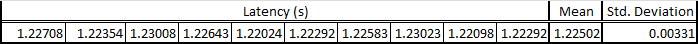
\includegraphics[scale=0.75]{../Logs/Instantiation.png}}
\caption{The time taken in seconds to instantiate 22 precomputed fragments over 10 runs.}
\label{fig:4.8}
\end{figure}
\end{comment}

\clearpage
\subsection{Simple Object}

Both methods were tested with a simple scene in which a sphere consisting of 760 triangles underwent a single collision.

\FloatBarrier

\subsubsection{Latency}

Meshinator has a negligible latency when fracturing an object with a low triangle count.

DVF has a much higher, noticeable latency when fracturing an object with a low triangle count. This is because the complexity is also bounded to the voxel resolution as well as triangle density. This is confirmed by the fact that the highest latency pipeline stages are the voxel partitioning and marching tetrahedra.

The standard deviation for the mean total time for DVF is higher than for Meshinator. This is because Meshinator always produces identical fragments each time\footnote{See Section~\ref{sect:acc}} whereas the proposed solution produces different fragments as well as a varying number of fragments.

\FloatBarrier

\begin{comment}
\begin{figure}[h!]
\centerline{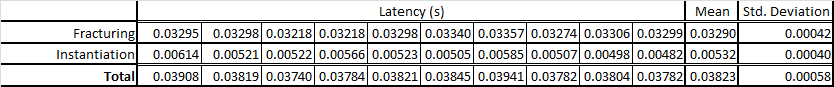
\includegraphics[scale=0.75]{../Logs/Fracture_Single_Sphere/Latency.png}}
\caption{The time taken in seconds to fracture a sphere consisting of 760 triangles over 10 runs using Meshinator.}
\label{fig:4.9}
\end{figure}

\begin{figure}[h!]
\centerline{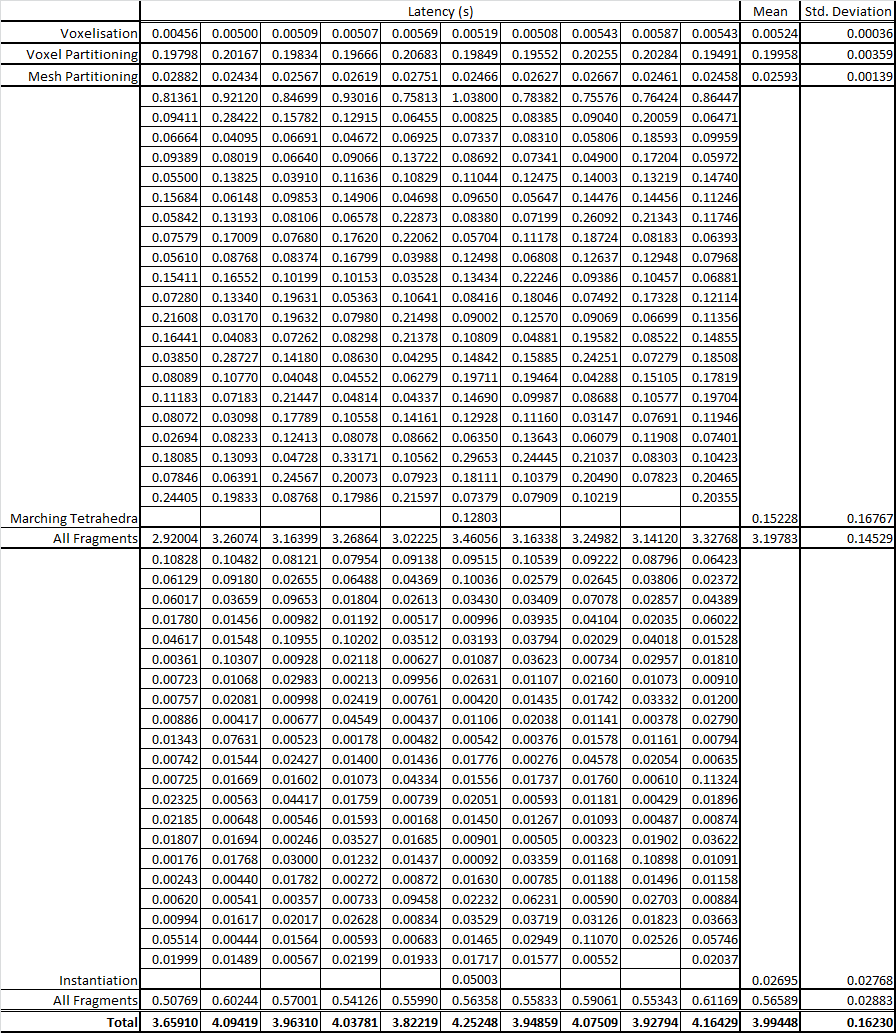
\includegraphics[scale=0.75]{../Logs/Voxel_Single_Sphere/Latency.png}}
\caption{The mean time taken by each pipeline stage in seconds when fracturing a sphere consisting of 760 triangles over 10 runs using DVF. The marching tetrahedra and instantiation stages are averaged over all fragments generated. Figure~\ref{fig:A.1} shows the full table.}
\label{fig:4.10}
\end{figure}
\end{comment}

\begin{figure}[h!]
\centerline{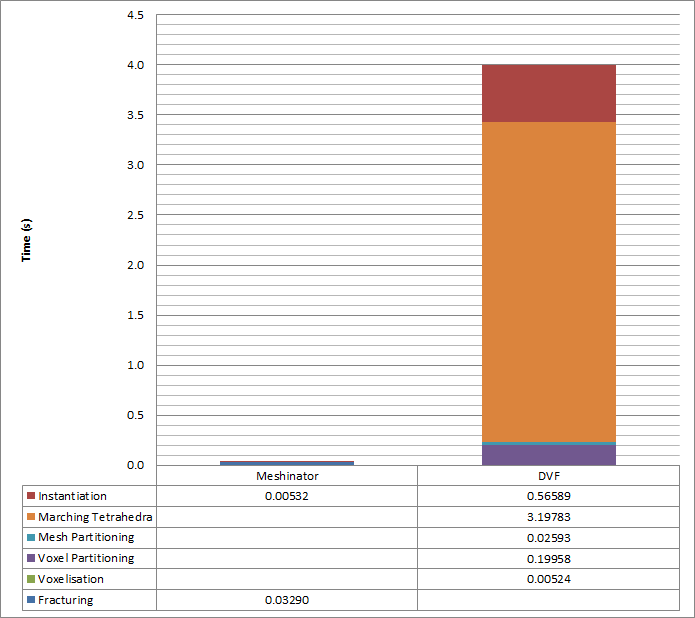
\includegraphics[scale=0.75]{../Logs/single_sphere_latency.png}}
\caption{The mean time taken by each pipeline stage in seconds when fracturing a sphere consisting of 760 triangles over 10 runs. Figures \ref{fig:A.1.1} and \ref{fig:A.1} show the full tables.}
\label{fig:4.10.1}
\end{figure}

\FloatBarrier

\begin{comment}

\subsubsection{GPU Usage}

GPU usage is well within the reasonable limits in both cases for fracturing a simple object.

\FloatBarrier

\begin{figure}[h!]
\centerline{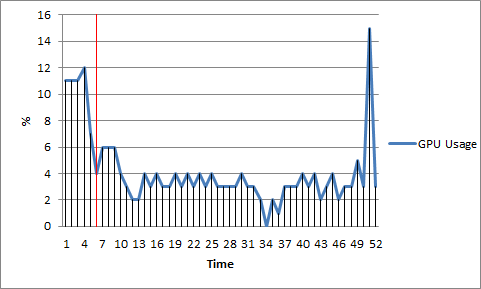
\includegraphics[scale=1.0]{../Logs/Fracture_Single_Sphere/GPU.png}}
\caption{The percentage GPU load taken over 100ms intervals when fracturing a sphere consisting of 760 triangles using Meshinator. The red line indicates the collision time.}
\label{fig:4.11}
\end{figure}

\begin{figure}[h!]
\centerline{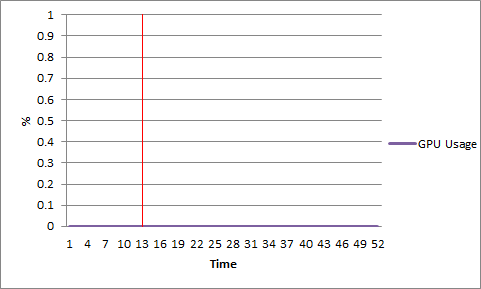
\includegraphics[scale=1.0]{../Logs/Voxel_Single_Sphere/GPU.png}}
\caption{The percentage GPU load taken over 100ms intervals when fracturing a sphere consisting of 760 triangles using DVF. The red line indicates the collision time.}
\label{fig:4.12}
\end{figure}

\FloatBarrier

\end{comment}

\clearpage
\subsubsection{Framerate}

Both solutions have an excellent framerate of $~120$ frames per second before and after the collision.

Meshinator does not have a complete framerate drop to 0 whereas DVF does. This is likely to be because Meshinator has multi-threaded components whereas DVF does not. Also, the instantiation overhead will be lower for Meshinator as it only created two fragments, DVF created 22.

Overall, Meshinator spends less time below 120 frames per second.

\FloatBarrier

\begin{comment}
\begin{figure}[h!]
\centerline{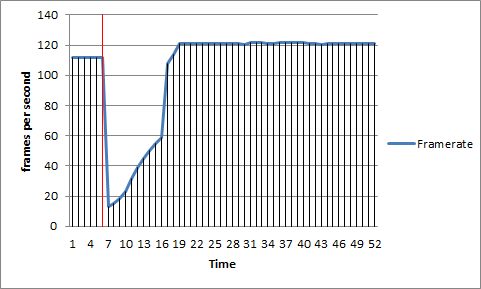
\includegraphics[scale=1.0]{../Logs/Fracture_Single_Sphere/FPS.png}}
\caption{The framerate taken over 100ms intervals when fracturing a sphere consisting of 760 triangles using Meshinator. The red line indicates the collision time.}
\label{fig:4.13}
\end{figure}

\begin{figure}[h!]
\centerline{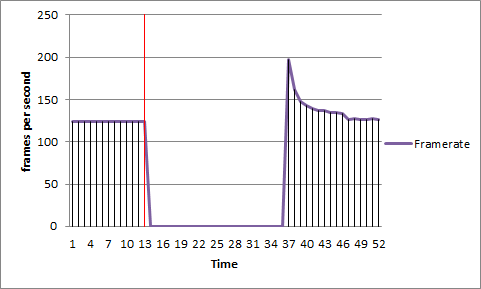
\includegraphics[scale=1.0]{../Logs/Voxel_Single_Sphere/FPS.png}}
\caption{The framerate taken over 100ms intervals when fracturing a sphere consisting of 760 triangles using DVF. The red line indicates the collision time.}
\label{fig:4.14}
\end{figure}
\end{comment}

\begin{figure}[h!]
\centerline{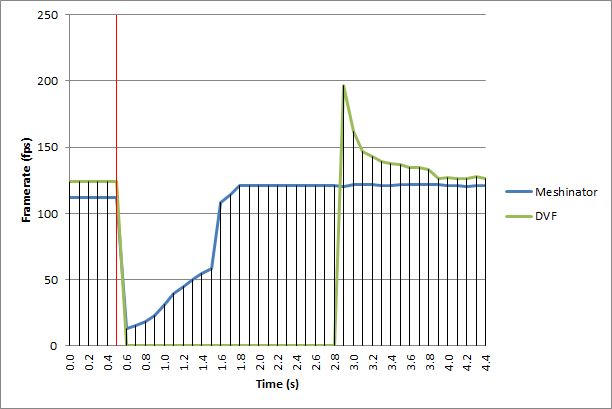
\includegraphics[scale=1.0]{../Logs/single_sphere_framerate.png}}
\caption{The framerate when fracturing a sphere consisting of 760 triangles. The red line indicates the collision time.}
\label{fig:4.14.1}
\end{figure}

\FloatBarrier

\clearpage
\subsubsection{Frametime}

As would be expected, in both cases there is a frametime spike after the collision as more work has to be done per frame as the object is fragmented.

DVF has a longer period between the collision and frametime spike and there are no frames produced at all before the pipeline is complete.

\FloatBarrier

\begin{comment}
\begin{figure}[h!]
\centerline{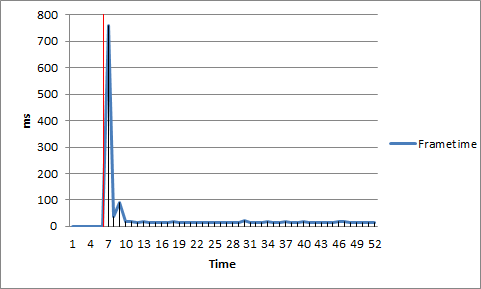
\includegraphics[scale=1.0]{../Logs/Fracture_Single_Sphere/Frametime.png}}
\caption{The frametime taken over 100ms intervals when fracturing a sphere consisting of 760 triangles using Meshinator. The red line indicates the collision time.}
\label{fig:4.15}
\end{figure}

\begin{figure}[h!]
\centerline{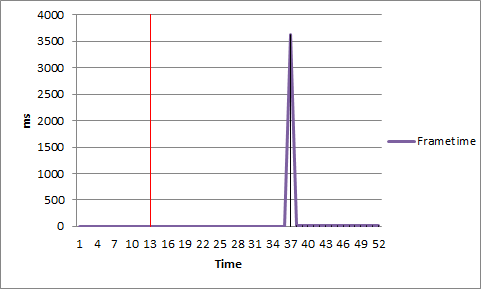
\includegraphics[scale=1.0]{../Logs/Voxel_Single_Sphere/Frametime.png}}
\caption{The frametime taken over 100ms intervals when fracturing a sphere consisting of 760 triangles using DVF. The red line indicates the collision time.}
\label{fig:4.16}
\end{figure}
\end{comment}

\begin{figure}[h!]
\centerline{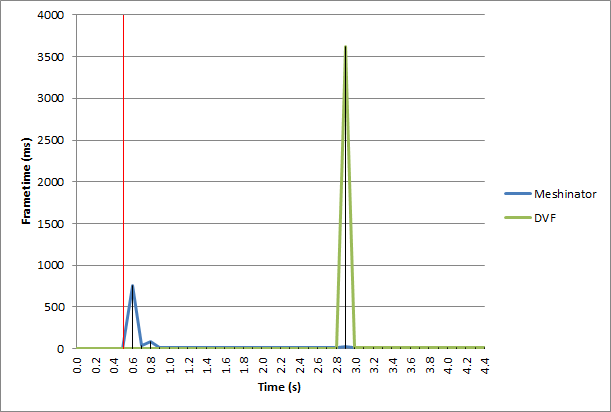
\includegraphics[scale=1.0]{../Logs/single_sphere_frametime.png}}
\caption{The frametime when fracturing a sphere consisting of 760 triangles. The red line indicates the collision time.}
\label{fig:4.16.1}
\end{figure}

\FloatBarrier

\clearpage
\subsection{Complex Object}

Both methods were tested with a simple scene in which the Stanford Bunny, consisting of 69,666 triangles, underwent a single collision.

\FloatBarrier

\subsubsection{Latency}

When fragmenting a higher triangle density object, Meshinator begins to have a noticeable latency, however, this is likely due to the instantiation overhead. Though an increase in latency would be expected with more complex objects as the complexity is bound to the number of triangles.

As expected, DVF has a much higher latency when fragmenting complex objects. The mesh partitioning stage now attributes to much more of this latency, with the voxel partitioning stage only having a slight increase. This is because the former is bound to the number of triangles whereas the latter is bound to voxel resolution, which has not increased much compared to the simple sphere. The instantiation phase now has a much higher standard deviation as the triangle density of the outer fragments (those that contain portions of the original mesh) is much higher than in the sphere case. The triangle density of the inner fragments is relatively unchanged as this depends on the voxel resolution.

\subsubsection{Framerate}

The framerate over time progresses in much the same way as with the simple object, however in both cases the period before regaining 120 frames per second is longer.

Meshinator now has a full drop to 0 frames per second. This is likely due to the instantiation overhead as the two fragments being created are of higher triangle complexity. 

\subsubsection{Frametime}

Frametime is as it was with the simple object, however the period between the collision and the spike is longer as would be expected.

\FloatBarrier

\begin{comment}
\begin{figure}[h!]
\centerline{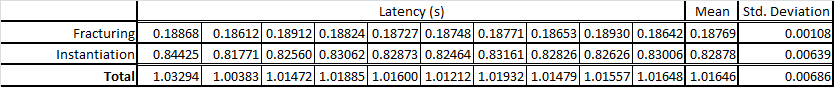
\includegraphics[scale=0.75]{../Logs/Fracture_Single_Bunny/Latency.png}}
\caption{The time taken in seconds to fracture the Stanford Bunny, consisting of 69,666 triangles, over 10 runs using Meshinator.}
\label{fig:4.17}
\end{figure}

\begin{figure}[h!]
\centerline{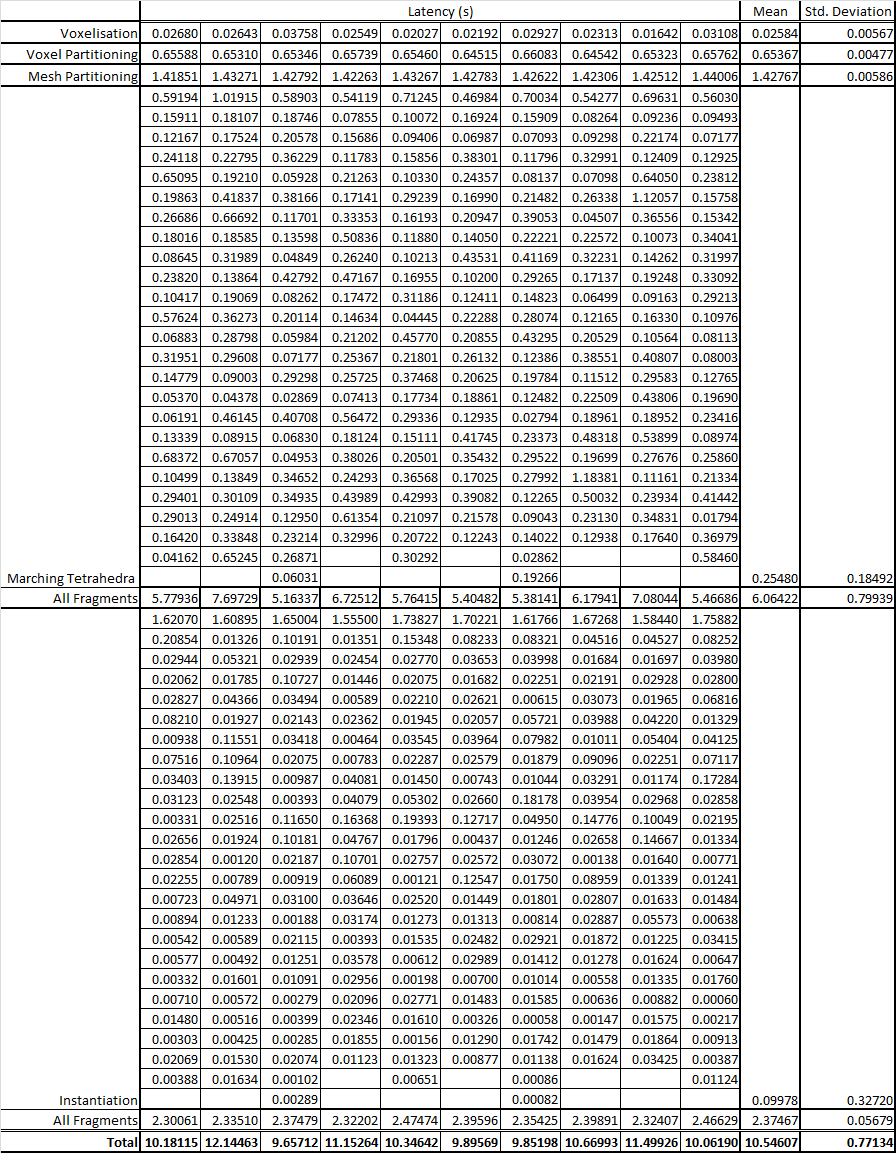
\includegraphics[scale=0.75]{../Logs/Voxel_Single_Bunny/Latency.png}}
\caption{The mean time taken by each pipeline stage in seconds when fracturing the Stanford Bunny, consisting of 69,666 triangles, over 10 runs using DVF. The marching tetrahedra and instantiation stages are averaged over all fragments generated. Figure~\ref{fig:A.2} shows the full table.}
\label{fig:4.18}
\end{figure}
\end{comment}

\begin{figure}[h!]
\centerline{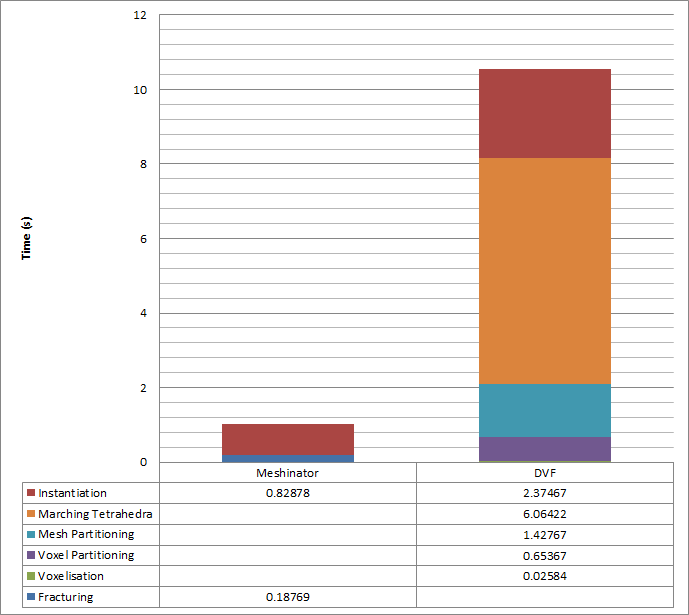
\includegraphics[scale=0.95]{../Logs/single_bunny_latency.png}}
\caption{The mean time taken by each pipeline stage in seconds when fracturing the Stanford Bunny, consisting of 69,666 triangles, over 10 runs. Figures \ref{fig:A.2.1} and \ref{fig:A.2} show the full tables.}
\label{fig:4.18.1}
\end{figure}

\FloatBarrier

\begin{comment}

\subsubsection{GPU Usage}

Both solutions have a reasonable GPU usage when fragmenting a complex object.

\FloatBarrier

\begin{figure}[h!]
\centerline{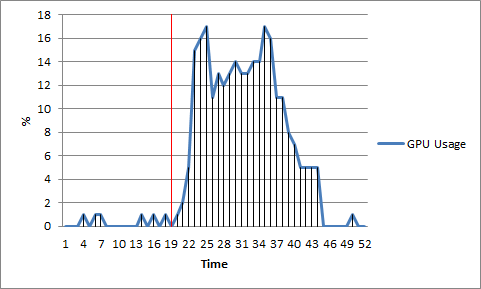
\includegraphics[scale=1.0]{../Logs/Fracture_Single_Bunny/GPU.png}}
\caption{The percentage GPU load taken over 100ms intervals when fracturing the Stanford Bunny, consisting of 69,666 triangles, using Meshinator. The red line indicates the collision time.}
\label{fig:4.19}
\end{figure}

\begin{sidewaysfigure}[h!]
\centerline{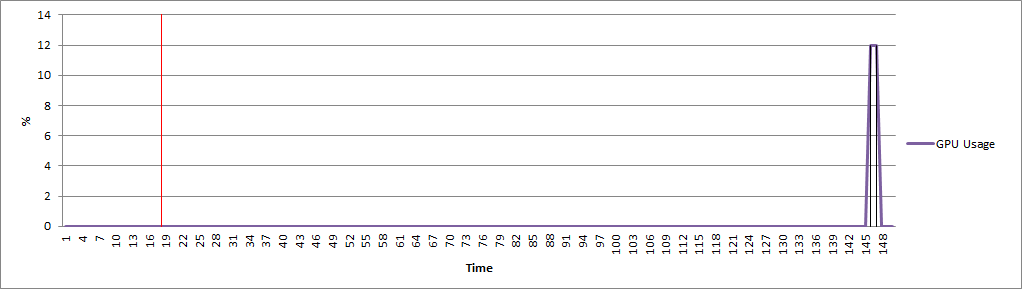
\includegraphics[scale=0.9]{../Logs/Voxel_Single_Bunny/GPU.png}}
\caption{The percentage GPU load taken over 100ms intervals when fracturing the Stanford Bunny, consisting of 69,666 triangles, using DVF. The red line indicates the collision time.}
\label{fig:4.20}
\end{sidewaysfigure}

\FloatBarrier

\end{comment}

\FloatBarrier

\begin{comment}
\begin{figure}[h!]
\centerline{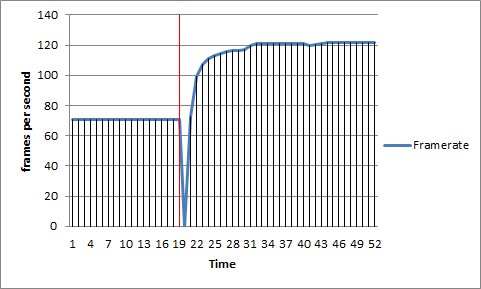
\includegraphics[scale=1.0]{../Logs/Fracture_Single_Bunny/FPS.png}}
\caption{The framerate taken over 100ms intervals when fracturing the Stanford Bunny, consisting of 69,666 triangles, using Meshinator. The red line indicates the collision time.}
\label{fig:4.21}
\end{figure}

\begin{sidewaysfigure}[h!]
\centerline{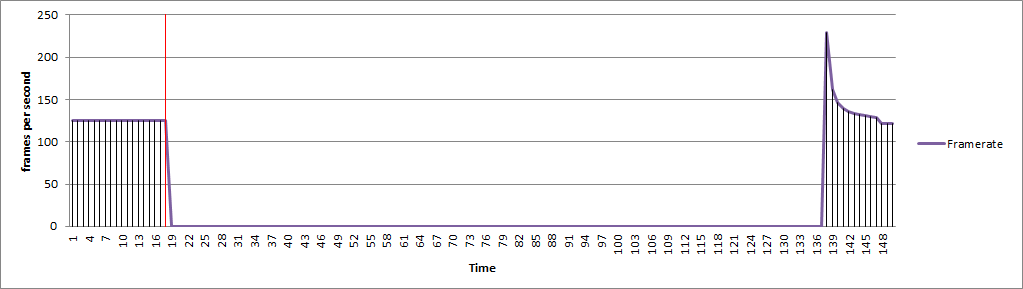
\includegraphics[scale=0.9]{../Logs/Voxel_Single_Bunny/FPS.png}}
\caption{The framerate taken over 100ms intervals when fracturing the Stanford Bunny, consisting of 69,666 triangles, using DVF. The red line indicates the collision time.}
\label{fig:4.22}
\end{sidewaysfigure}
\end{comment}

\begin{sidewaysfigure}[h!]
\centerline{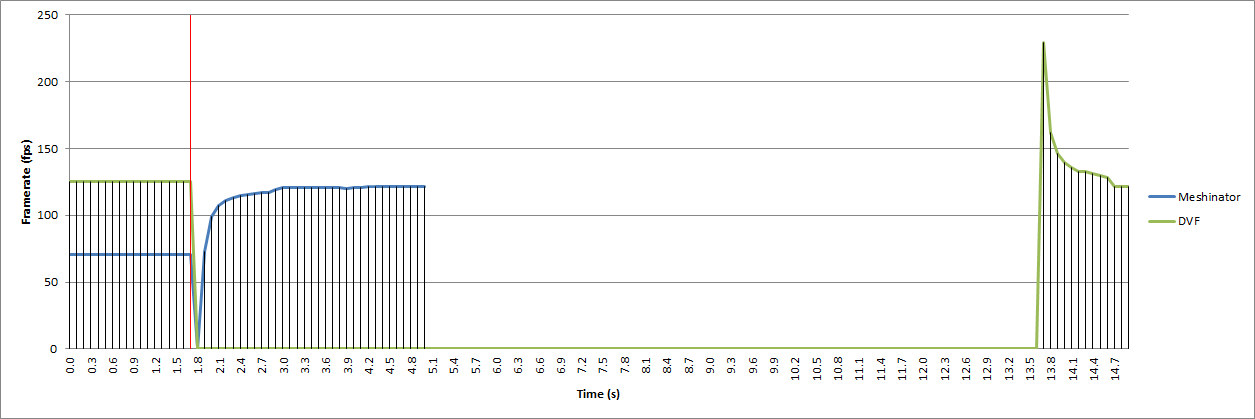
\includegraphics[scale=0.7]{../Logs/single_bunny_framerate.png}}
\caption{The framerate when fracturing the Stanford Bunny, consisting of 69,666 triangles. The red line indicates the collision time.}
\label{fig:4.22.1}
\end{sidewaysfigure}

\FloatBarrier

\FloatBarrier

\begin{comment}
\begin{figure}[h!]
\centerline{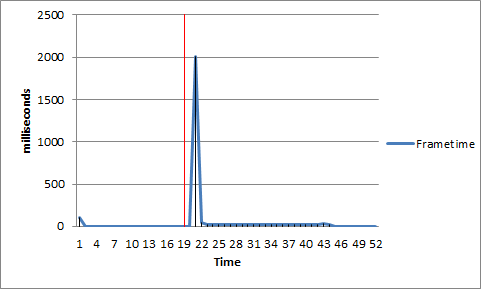
\includegraphics[scale=1.0]{../Logs/Fracture_Single_Bunny/Frametime.png}}
\caption{The frametime taken over 100ms intervals when fracturing the Stanford Bunny, consisting of 69,666 triangles, using Meshinator. The red line indicates the collision time.}
\label{fig:4.23}
\end{figure}

\begin{sidewaysfigure}[h!]
\centerline{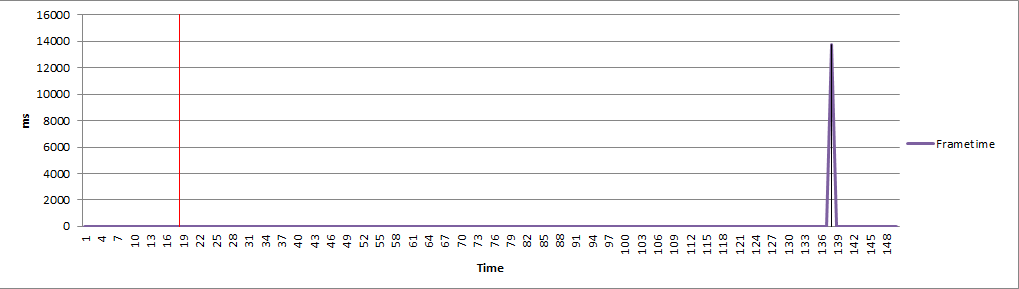
\includegraphics[scale=0.9]{../Logs/Voxel_Single_Bunny/Frametime.png}}
\caption{The frametime taken over 100ms intervals when fracturing the Stanford Bunny, consisting of 69,666 triangles, using DVF. The red line indicates the collision time.}
\label{fig:4.24}
\end{sidewaysfigure}
\end{comment}

\begin{sidewaysfigure}[h!]
\centerline{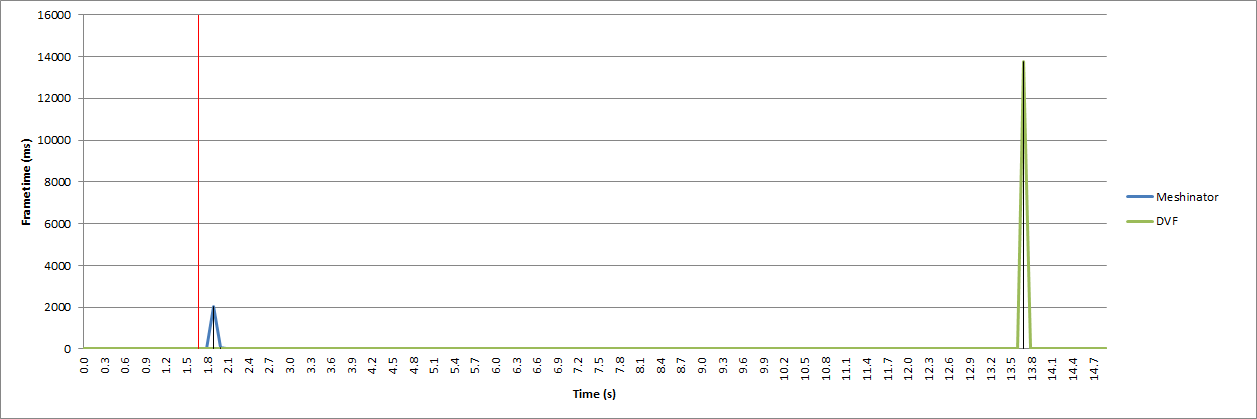
\includegraphics[scale=0.7]{../Logs/single_bunny_frametime.png}}
\caption{The frametime when fracturing the Stanford Bunny, consisting of 69,666 triangles. The red line indicates the collision time.}
\label{fig:4.24.1}
\end{sidewaysfigure}

\FloatBarrier

\clearpage
\subsection{Multiple Objects}

Both methods were tested with a simple scene in which two Stanford Bunnies each underwent a single collision simultaneously.

\FloatBarrier

\subsubsection{Latency}

In both cases the latency has roughly doubled as the number of objects has.

The standard deviation for the total time has not increased significantly for Meshinator, again because the fragments are always identical. For DVF it has increased as would be expected.

\subsubsection{Framerate}

Framerate follows the same trend as before in both cases, with the period where no frames are being produced having increased as mean total latency did.

\subsubsection{Frametime}

Frametime is as with the previous two test cases, with the period before the frametime spike increasing as the number of objects has.

It is still important to note that, though the frametime is 0, there are still no frames being produced between the collision and the spike, as shown by the framerate graph.

\FloatBarrier

\begin{comment}
\begin{figure}[h!]
\centerline{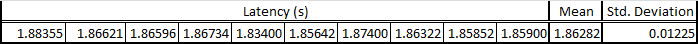
\includegraphics[scale=0.75]{../Logs/Fracture_Two_Bunny/Latency.png}}
\caption{The time taken in seconds to simultaneously fracture two Stanford Bunnies, each consisting of 69,666 triangles, over 10 runs using Meshinator.}
\label{fig:4.25}
\end{figure}

\begin{figure}[h!]
\centerline{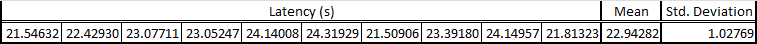
\includegraphics[scale=0.75]{../Logs/Voxel_Two_Bunny/Latency.png}}
\caption{The time taken in seconds to simultaneously fracture two Stanford Bunnies, each consisting of 69,666 triangles, over 10 runs using DVF.}
\label{fig:4.25}
\end{figure}
\end{comment}

\begin{figure}[h!]
\centerline{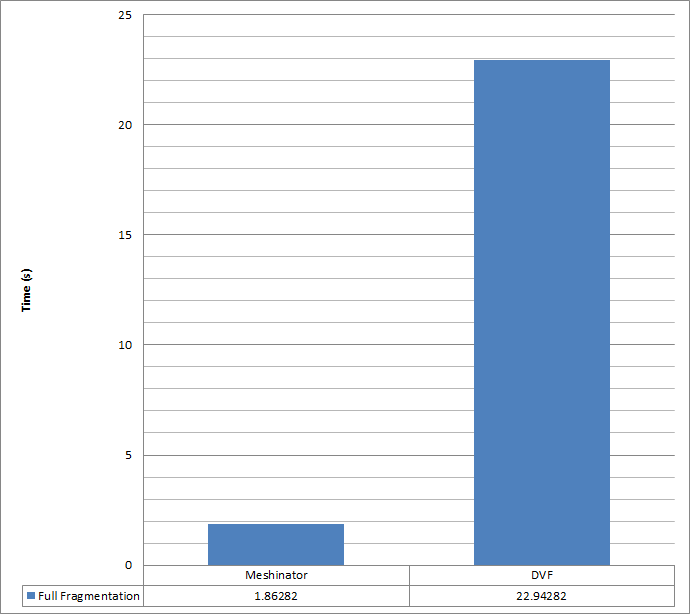
\includegraphics[scale=0.95]{../Logs/double_bunny_latency.png}}
\caption{The time taken in seconds to simultaneously fracture two Stanford Bunnies, each consisting of 69,666 triangles, over 10 runs. Figures \ref{fig:A.3.1} and \ref{fig:A.3} show the full tables.}
\label{fig:4.25}
\end{figure}

\FloatBarrier

\begin{comment}

\subsubsection{GPU Usage}

Both solutions have a reasonable GPU usage when fragmenting two complex objects.

\FloatBarrier

\begin{figure}[h!]
\centerline{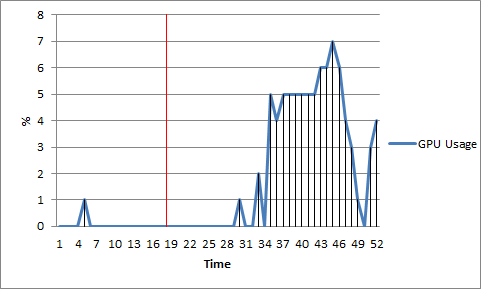
\includegraphics[scale=1.0]{../Logs/Fracture_Two_Bunny/GPU.png}}
\caption{The percentage GPU load taken over 100ms intervals when simultaneously fracturing two Stanford Bunnies, each consisting of 69,666 triangles, using Meshinator. The red line indicates the collision time.}
\label{fig:4.26}
\end{figure}

\begin{sidewaysfigure}[h!]
\centerline{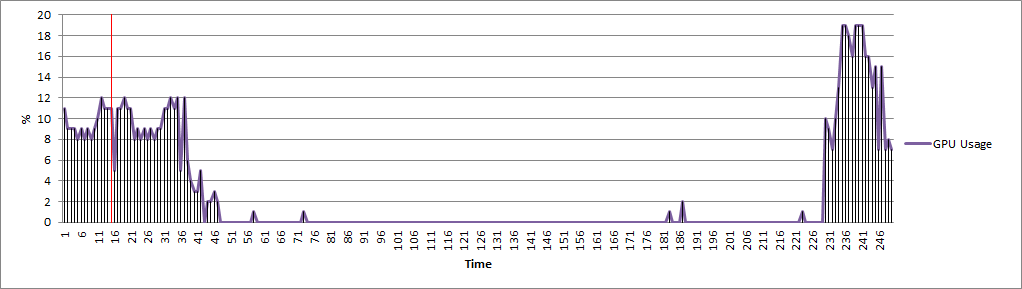
\includegraphics[scale=0.9]{../Logs/Voxel_Two_Bunny/GPU.png}}
\caption{The percentage GPU load taken over 100ms intervals when simultaneously fracturing two Stanford Bunnies, each consisting of 69,666 triangles, using DVF. The red line indicates the collision time.}
\label{fig:4.27}
\end{sidewaysfigure}

\FloatBarrier

\end{comment}

\begin{comment}
\begin{figure}[h!]
\centerline{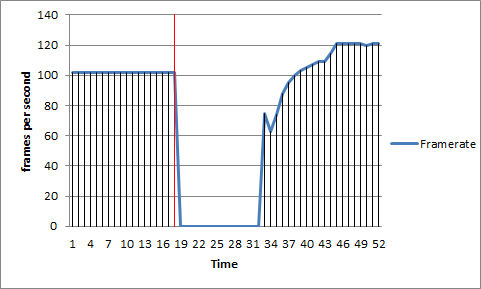
\includegraphics[scale=1.0]{../Logs/Fracture_Two_Bunny/FPS.png}}
\caption{The framerate taken over 100ms intervals when simultaneously fracturing two Stanford Bunnies, each consisting of 69,666 triangles, using Meshinator. The red line indicates the collision time.}
\label{fig:4.28}
\end{figure}

\begin{sidewaysfigure}[h!]
\centerline{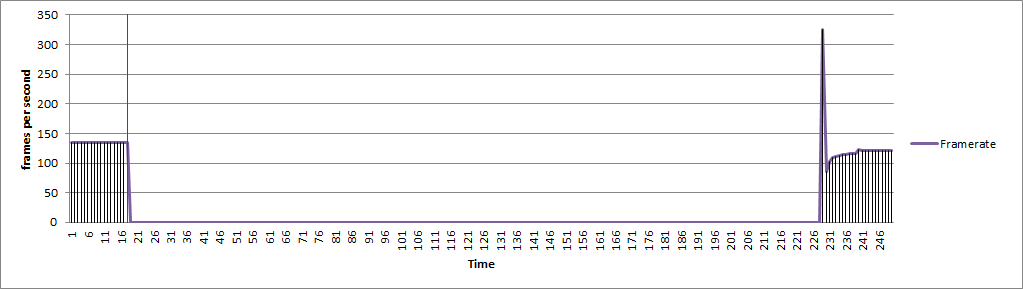
\includegraphics[scale=0.9]{../Logs/Voxel_Two_Bunny/FPS.png}}
\caption{The framerate taken over 100ms intervals when simultaneously fracturing two Stanford Bunnies, each consisting of 69,666 triangles, using DVF. The red line indicates the collision time.}
\label{fig:4.29}
\end{sidewaysfigure}
\end{comment}

\begin{sidewaysfigure}[h!]
\centerline{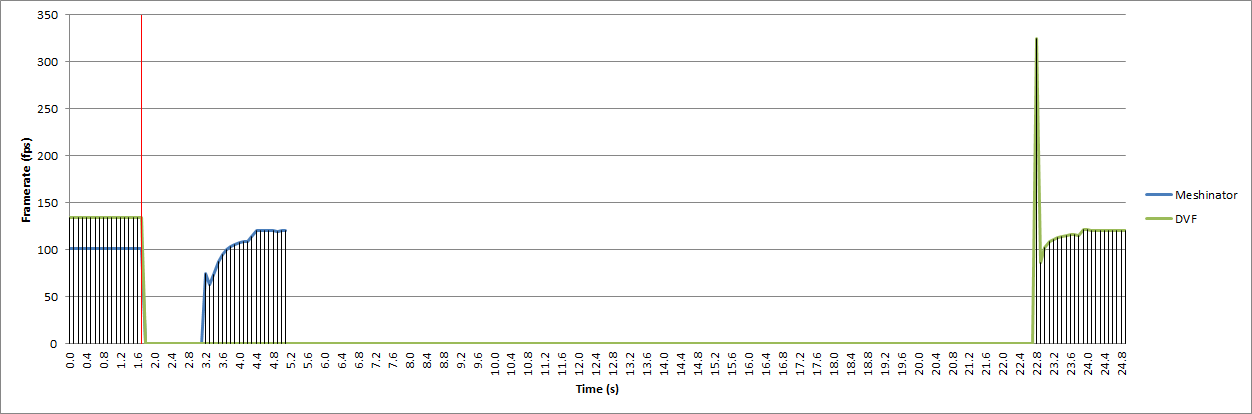
\includegraphics[scale=0.7]{../Logs/double_bunny_framerate.png}}
\caption{The framerate when simultaneously fracturing two Stanford Bunnies, each consisting of 69,666 triangles. The red line indicates the collision time.}
\label{fig:4.29.1}
\end{sidewaysfigure}

\FloatBarrier

\FloatBarrier

\begin{comment}
\begin{figure}[h!]
\centerline{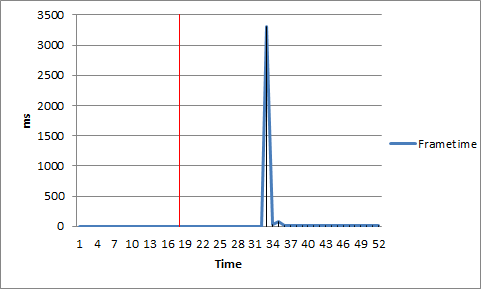
\includegraphics[scale=1.0]{../Logs/Fracture_Two_Bunny/Frametime.png}}
\caption{The frametime taken over 100ms intervals when simultaneously fracturing two Stanford Bunnies, each consisting of 69,666 triangles, using Meshinator. The red line indicates the collision time.}
\label{fig:4.30}
\end{figure}

\begin{sidewaysfigure}[h!]
\centerline{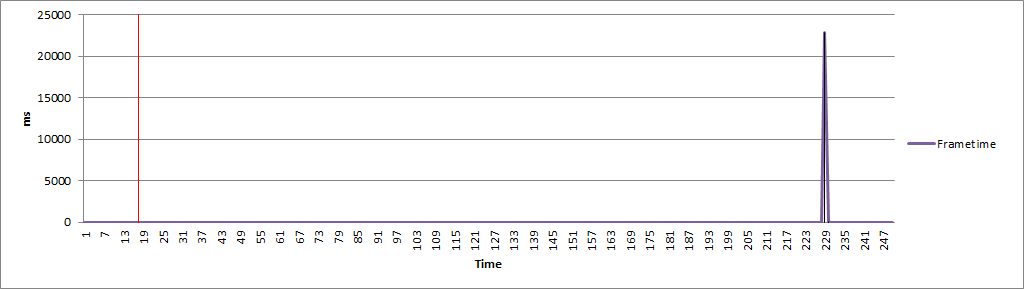
\includegraphics[scale=0.9]{../Logs/Voxel_Two_Bunny/Frametime.png}}
\caption{The frametime taken over 100ms intervals when simultaneously fracturing two Stanford Bunnies, each consisting of 69,666 triangles, using DVF. The red line indicates the collision time.}
\label{fig:4.31}
\end{sidewaysfigure}
\end{comment}

\begin{sidewaysfigure}[h!]
\centerline{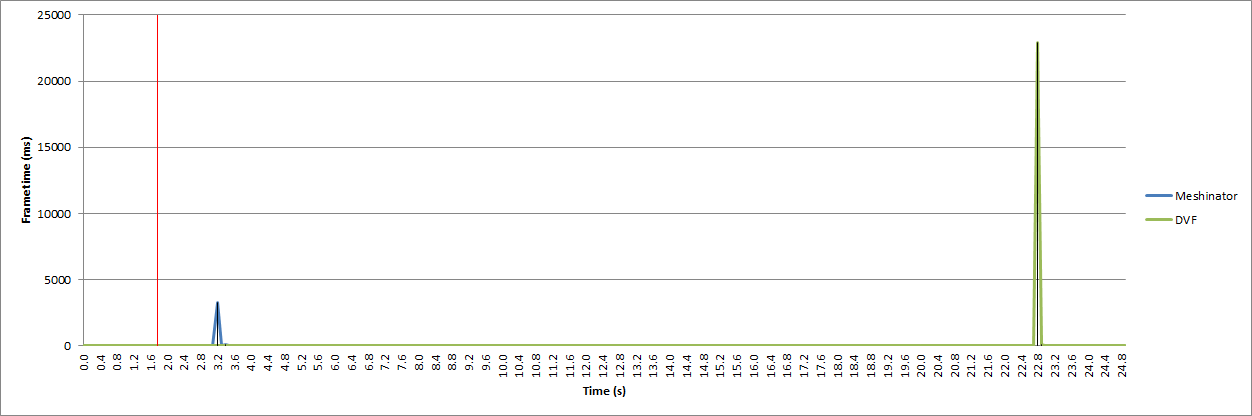
\includegraphics[scale=0.7]{../Logs/double_bunny_frametime.png}}
\caption{The frametime when simultaneously fracturing two Stanford Bunnies, each consisting of 69,666 triangles. The red line indicates the collision time.}
\label{fig:4.31.1}
\end{sidewaysfigure}

\FloatBarrier

\subsection{Results}

\label{sect:results}

It is clear from these results that Dynamic Volumetric Fragmentation is not feasible for a real-time application in its current state. Even if the instantiation overhead were not present, there is too much latency in the other pipeline stages. 

The Meshinator library would also not be usable in a realtime situation based on the results seen in the complex and multi-object trials. However a much greater proportion of the observed latency is due to instantiation than is the case for DVF. Furthermore, M\"{u}ller, Chentanez and Tae-Yong demonstrate that real-time fragmentation can be achieved even if Meshinator is not a suitable example\cite{Muller:2013:RTD:2461912.2461934}.

Meshinator likely outperformed DVF in these empirical tests for the following reasons:

\begin{enumerate}
\item{The plane intersection method is only bounded in time complexity by the number of triangles. DVF is also bounded by voxel density which is independent of object triangle complexity.}
\item{Meshinator only produces two fragments per collision which reduces the work done to produce the fragment meshes as well as instantiate them. DVF produces a variable number of fragments.}
\label{point:number}
\item{Meshinator produces fragments with shear surfaces reducing the triangle complexity of the fragments. DVF creates noisy surfaces.}
\label{point:smooth}
\item{Meshinator is fully multi-threaded. DVF is not.}
\label{point:multi}
\end{enumerate}

Whilst Points \ref{point:number} and \ref{point:smooth} reduce the time complexity of Meshinator, they also reduce its functionality. DVF is much less strict in what it is capable of producing and so can achieve more accurate and varied fragmentations which depend better on the physical attributes of the solid.

Point \ref{point:multi} will be addressed in Section~\ref{sect:multi}.

\FloatBarrier

\section{Requirements Met}

The requirements, originally stated in Section~\ref{sect:req}, are enumerated below alongside evidence of their completion:

\begin{enumerate}
\item{The solution \emph{must} enable a scene in which an object of reasonable complexity\footnote{Such as the Stanford Bunny} is fragmented in a manner which resembles a real world interaction as closely as possible. Demonstrated in Section~\ref{sect:result}}
\label{point:complex}
\item{The solution \emph{must} be object independent. That is any object may be made destructible without retroactively altering the object's definition.  Demonstrated in Section~\ref{sect:result}}
\label{point:independant}
\item{The solution \emph{must} take into account the defined physical characteristics of the object to be fragmented as well as those defined by the collision when resolving.  Demonstrated in Sections \ref{sect:pre} and \ref{sect:destr}}
\label{point:physics}

\item{The solution \emph{should} produce fragments with the correct physical properties based on those of the original object and the size of the each given fragment.  Demonstrated in Section~\ref{sect:postphysics}}
\label{point:properties}
\item{The solution \emph{should} not produce fragments with unconnected islands.  Demonstrated in Section~\ref{sect:islands}}
\label{point:islands}

\item{The solution \emph{could} run in real-time.}
\label{point:realtime}

\item{The solution \emph{won't} deal with texture mapping onto fragments.}
\label{point:texture}
\item{The solution \emph{won't} deal with structural integrity.}
\label{point:structure}
\end{enumerate}

Point~\ref{point:realtime} unfortunately has not been achieved as stated in Section~\ref{sect:results}. Further work that could be done to address this is explored in Section~\ref{sect:multi}.

As expected, neither Point \ref{point:texture} or \ref{point:structure} were achieved.

\section{Feasible Continuations}

\label{sect:cont}

Two areas for improvement are explored below.

\subsection{Accuracy}

\label{sect:accurate}

The fragmentation method used, while producing visually pleasing results compared to Meshinator\footnote{Though the blocky structure is probably more visible than would be desired.}, is not as physically accurate as Dynamic Volumetric Fragmentation can allow.

Because the object is being modelled as a solid volume it would be possible to write much more complex algorithms which fully simulate how impact force should be propagated internally as well as how the cracks should form. This is the biggest strength of DVF.

As the pipeline stages are well encapsulated, it would also be possible to have different algorithms for different materials and use the correct one on an object by object basis.

\subsection{Parallelism}

\label{sect:multi}

In its current state, none of the pipeline is parallelised. There are two ways in which this could be improved.

\subsubsection{Coarse-grained}

Currently the entire pipeline runs in the same thread as the Unity3D physics engine which causes the whole scene to pause while the fragmentation resolves. Had time allowed, the pipeline would have been moved to its own thread to prevent this. Unity3D has many thread-unsafe areas and all of the stages were developed without such areas meaning that they could be used in a multi-threaded environment.

Only moving the whole pipeline to its own thread does not solve the latency problem however. Even if the stages are executing independently of the physics engine, allowing it to continue to progress, if they are not all complete between the time the collision is predicted\footnote{See Section~\ref{sect:pre}} and the collision then the fragments will not interact with the colliding object as is required. Simply increasing the radius of collision prediction does not work as that will mean the assumptions made in Section~\ref{sect:pre} no longer hold.

\subsubsection{Fine-grained}

Within each pipeline stage, most operations are being performed on vertices or voxels independent of the results on the previous vertices or voxel. This would allow massive parallelism to be exploited on the GPU for these operations.

GPU parallelisation is the best option for allowing DVF to be viable for a real-time application. This would have been explored had time allowed.

\section{Conclusion}

The advantages and disadvantages of Dynamic Volumetric Fragmentation have been investigated with comparison to another solution. While it was found that DVF would not currently be suitable for a real-time application, possible continuations which would address this have been discussed, primarily involving parallelisation that could not be completed due to time constraints.

An argument has been made for the merits of using a volumetric approach to physics based destruction. It is suggested that the current partitioning algorithm could be replaced with one featuring higher physical accuracy which would improve the already pleasing visual results.